% Autor: Leonhard Segger, Alexander Neuwirth
% Datum: 2017-10-30
\documentclass[
	% Papierformat
	a4paper,
	% Schriftgröße (beliebige Größen mit „fontsize=Xpt“)
	12pt,
	% Schreibt die Papiergröße korrekt ins Ausgabedokument
	pagesize,
	% Sprache für z.B. Babel
	ngerman
]{scrartcl}

% Achtung: Die Reihenfolge der Pakete kann (leider) wichtig sein!
% Insbesondere sollten (so wie hier) babel, fontenc und inputenc (in dieser
% Reihenfolge) als Erstes und hyperref und cleveref (Reihenfolge auch hier
% beachten) als Letztes geladen werden!

% Silbentrennung etc.; Sprache wird durch Option bei \documentclass festgelegt
\usepackage{babel}
% Verwendung der Zeichentabelle T1 (Sonderzeichen etc.)
\usepackage[T1]{fontenc}
% Legt die Zeichenkodierung der Eingabedatei fest, z.B. UTF-8
\usepackage[utf8]{inputenc}
% Schriftart
\usepackage{lmodern}
% Zusätzliche Sonderzeichen
\usepackage{textcomp}

% Mathepaket (intlimits: Grenzen über/unter Integralzeichen)
\usepackage[intlimits]{amsmath}
% Ermöglicht die Nutzung von \SI{Zahl}{Einheit} u.a.
\usepackage{siunitx}
% Zum flexiblen Einbinden von Grafiken (\includegraphics)
\usepackage{graphicx}
% Abbildungen im Fließtext
\usepackage{wrapfig}
% Abbildungen nebeneinander (subfigure, subtable)
\usepackage{subcaption}
% Funktionen für Anführungszeichen
\usepackage{csquotes}
% Zitieren, Bibliographie
\usepackage{biblatex}


% Zur Darstellung von Webadressen
\usepackage{url}
%chemische Formeln
\usepackage[version=4]{mhchem}
% siunitx: Deutsche Ausgabe, Messfehler getrennt mit ± ausgeben
\usepackage{floatrow}
\floatsetup[table]{capposition=top}
\usepackage{float}
% Verlinkt Textstellen im PDF-Dokument
\usepackage[unicode]{hyperref}
% "Schlaue" Referenzen (nach hyperref laden!)
\usepackage{cleveref}
\sisetup{
	locale=DE,
	separate-uncertainty
}
\bibliography{14Mo_A3_07-05-2018_References}

\begin{document}
	
	\begin{titlepage}
		\centering
		{\scshape\LARGE Versuchsbericht zu \par}
		\vspace{1cm}
		{\scshape\huge A3 - Absorption von Beta- und Gamma-Strahlung \par}
		\vspace{2.5cm}
		{\LARGE Gruppe 14Mo \par}
		\vspace{0.5cm}
		
		{\large Alexander Neuwirth (E-Mail: a\_neuw01@wwu.de) \par}
		{\large Leonhard Segger (E-Mail: l\_segg03@uni-muenster.de) \par}
		\vfill
		
		durchgeführt am 07.05.2018\par
		betreut von\par
		{\large Johann Preuß}  
		
		\vfill
		
		{\large \today\par}
	\end{titlepage}
	\tableofcontents
	\newpage

	\section{Kurzfassung}
	%TODO Hypothese	und deren Ergebnis, wenn Hypothese ist, dass nur Theorie erfüllt, sagen: Erwartung: Theorie aus einführung (mit reflink) erfüllt
	%TODO Ergebnisse, auch Zahlen, mindestens wenn's halbwegs Sinn ergibt
	%TODO Was wurde gemacht
	%TODO manche leute wollen Passiv oder "man", manche nicht
	In diesem Versuch wurde die Absorption von Beta- und Gammastrahlung untersucht. %überflüssig?
	Dazu wurde der Zusammenhang zwischen Schichtdicke eines Absorbers, Art der Strahlung des Präparats und Impulsrate betrachtet.
	Zunächst wurde die Zählrohrcharakteristik bestimmt, die, wie erwartet wurde, einen starken Anstieg der Impulsrate ab einer bestimmten Spannung und ein darauf folgendes Plateau enthält.
	Es wurde erwartet, dass die Menge der Impulse durch Untergrundstrahlung in einem festen Zeitintervall Poisson-verteilt ist.
	Dies konnte gezeigt werden.
	Für die Absorption von $\gamma$-Strahlung durch Blei war eine exponentielle Abnahme der Impulsrate mit der Schichtdicke des Absorbers zu erwarten.
	Dies ließ sich experimentell nachweisen.
	Es wurde ein Massenabsorptionskoeffizient von Blei von $\mu_{\gamma,m}$ = $\SI{0,0978+-0,0035}{cm^2/g}$ bestimmt und mithilfe eines Literaturwertes konnte die Größenordnung des Messwerts bestätigt werden.
	Bei der Absorption von $\beta$-Strahlung war gemäß der Einführung  eine exponentielle Abnahme nur für bestimmte Schichtdicken zu erwarten. \cite{Einfuehrung}
	Die Hypothese war hier, dass die gemessenen Schichtdicken von 0 bis \SI{215}{\micro \meter} Teil dieser bestimmten Schichtdicken sind, was der experimentelle Befund bestätigte.
	Hier wurde ein Massenabsorptionskoeffizient von Aluminium von $\mu_{\beta,m}$ = $\SI{7,2+-1,1}{cm^2/g}$
	Außerdem wurde die Absorption von $\beta$-Strahlung durch Gummi und Plexiglas untersucht.
	
	\section{Methoden}\label{Methoden}
	%TODO Bilder von der Website klauen
	Der Versuchsaufbau bestand aus einem Geiger-Müller-Zählrohr, das an ein Betriebsgerät angeschlossen war.
	Vor das Glimmerfenster des Zählrohrs konnten nun verschiedene radioaktive Präparate installiert werden und unterschiedliche Absorber zwischen Präparat und Zählrohr gebracht werden.
	
	Zunächst wurde die Charakteristik des Geiger-Müller-Zählrohres bestimmt, um die folgenden Untersuchungen im Plateaubereich der Zählrohrkennlinie durchführen zu können.
	Dazu wurde die Impulsrate des Zählrohrs mit $\beta$-Präparat bei steigender Zählrohrspannung bestimmt.
	Begonnen wurde hier unmittelbar unter der Einsatzspannung.
	Die folgenden Messungen wurden bei einer Betriebsspannung ca. \SI{100}{\volt} über der Einsatzspannung durchgeführt.
	
	Dann wurde, um die mittlere Untergrundaktivität zu bestimmen, 200 mal die Zahl der Untergrundimpulse in \SI{10}{\second} gemessen.
	Anschließend wurde die Impulsrate des $\gamma$-Präparats mit zunehmender Schichtdicke des Blei-Absorbers gemessen und die Impulsrate des $\beta$-Präparats mit zunehmender Aluminium-Absorber-Dicke.
	Zuletzt wurde noch die Impulsrate des $\beta$-Präparats mit Plexiglas- und Gummiabsorber bei konstanter Schichtdicke bestimmt.
	
	Hierbei wurden jeweils mindestens 1111 Impulse gemessen, um die relative Unsicherheit unter 3\% zu halten.
	Die Betriebsspannung wurde vom Betriebsgerät abgelesen und nicht mit einem externen Voltmeter überprüft.
	
	%TODO Bestimmen der Zählzeit => 1111 Impulse
	
	\section{Ergebnisse und Diskussion}
	%TODO Datenanalyse -> Überschrift?
	%TODO Unsicherheiten
	

	
	\subsection{Beobachtung und Datenanalyse}
	\subsubsection{Unsicherheiten} %TODO Schon alles?
	Die Unsicherheit der Betriebsspannung des Geiger-Müller-Zahlrohrs beträgt \SI{3}{V} (dreieckige WDF).  
	Die Zählzeit wurde in Sekunden auf einer Digitalanzeige gestoppt, wodurch sich eine Unsicherheit von \SI{0,6}{s} ergibt (rechteckige WDF).
	Wie in \cref{Methoden} beschrieben ist die relative Unsicherheit der Impulsmessungen kleiner 3\%.
	Die Bestimmung der Dicke der Absorber aus Blei hat eine Unsicherheit von \SI{0,12}{mm}, die sich zusammensetzt aus der Genauigkeit des Messschiebers und dem Fehler durch die ungleichmäßige Oberfläche des Materials.
	
	\subsubsection{Zählrohrcharakteristik}
	%TODO Einflüsse von veränderten Parametern auf Messung
	In \cref{Zaehlrohrcharakteristik} ist die Impulsrate gegen die Zählrohrspannung aufgetragen.
	Bei \SI{313+-7}{\volt} steigt die Impulsrate abrupt von 0 auf 9 Impulse pro Sekunde und ändert sich danach nur noch unwesentlich. 
	
	%TODO mehr!
	
	\begin{figure}[H]
		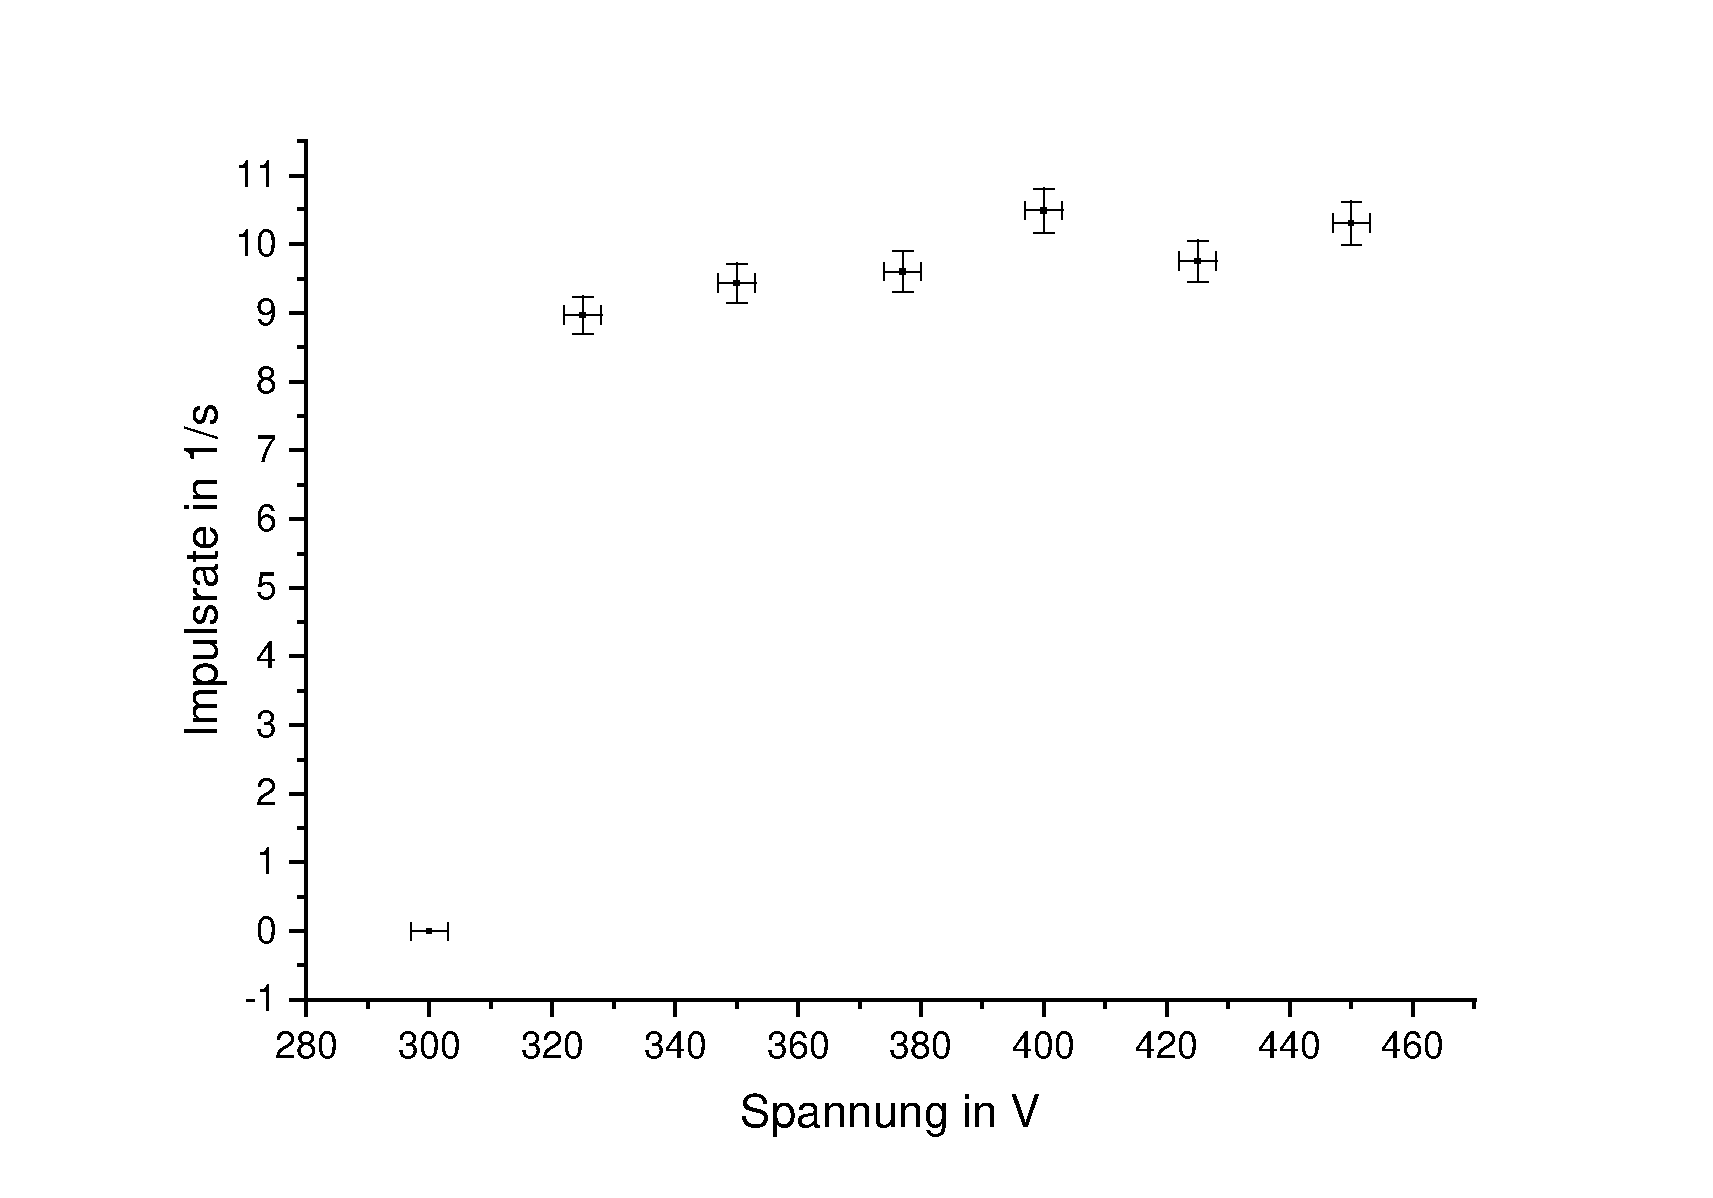
\includegraphics[width=0.7\textwidth]{Zaehlrohrcharakteristik}
		\centering
		\caption{Aufgenommene Zählrohrcharakteristik unter Verwendung eines $\beta$-Präparats.}%TODO Titel
		\label{Zaehlrohrcharakteristik}
		\centering
	\end{figure}
	
	\subsubsection{Untergrundpulse}
	Die Messung der Untergrundimpulse über 200 mal 10 Sekunden ergab einen Mittelwert von 2,685 Impulsen und eine Standardabweichung von 1,519. 
	In \cref{Untergrund} sind die absolute und die relative Häufigkeitsverteilung dargestellt.
	Da sich die Ordinatenwerte lediglich um einen Faktor von 200 unterscheiden, lässt sich an der linken Achse die absolute und an der rechten die relative Häufigkeit ablesen.
	Des Weiteren ist in \cref{Untergrund} die Poisson-Verteilung für $\bar{N}$ = 2,685 abgebildet.
	\begin{equation}
		\psi(N) = \frac{\bar{N}^N \cdot e^{(-\bar{N})}}{N!}
	\label{Poisson}
	\end{equation}
	
	\begin{figure}[H]
		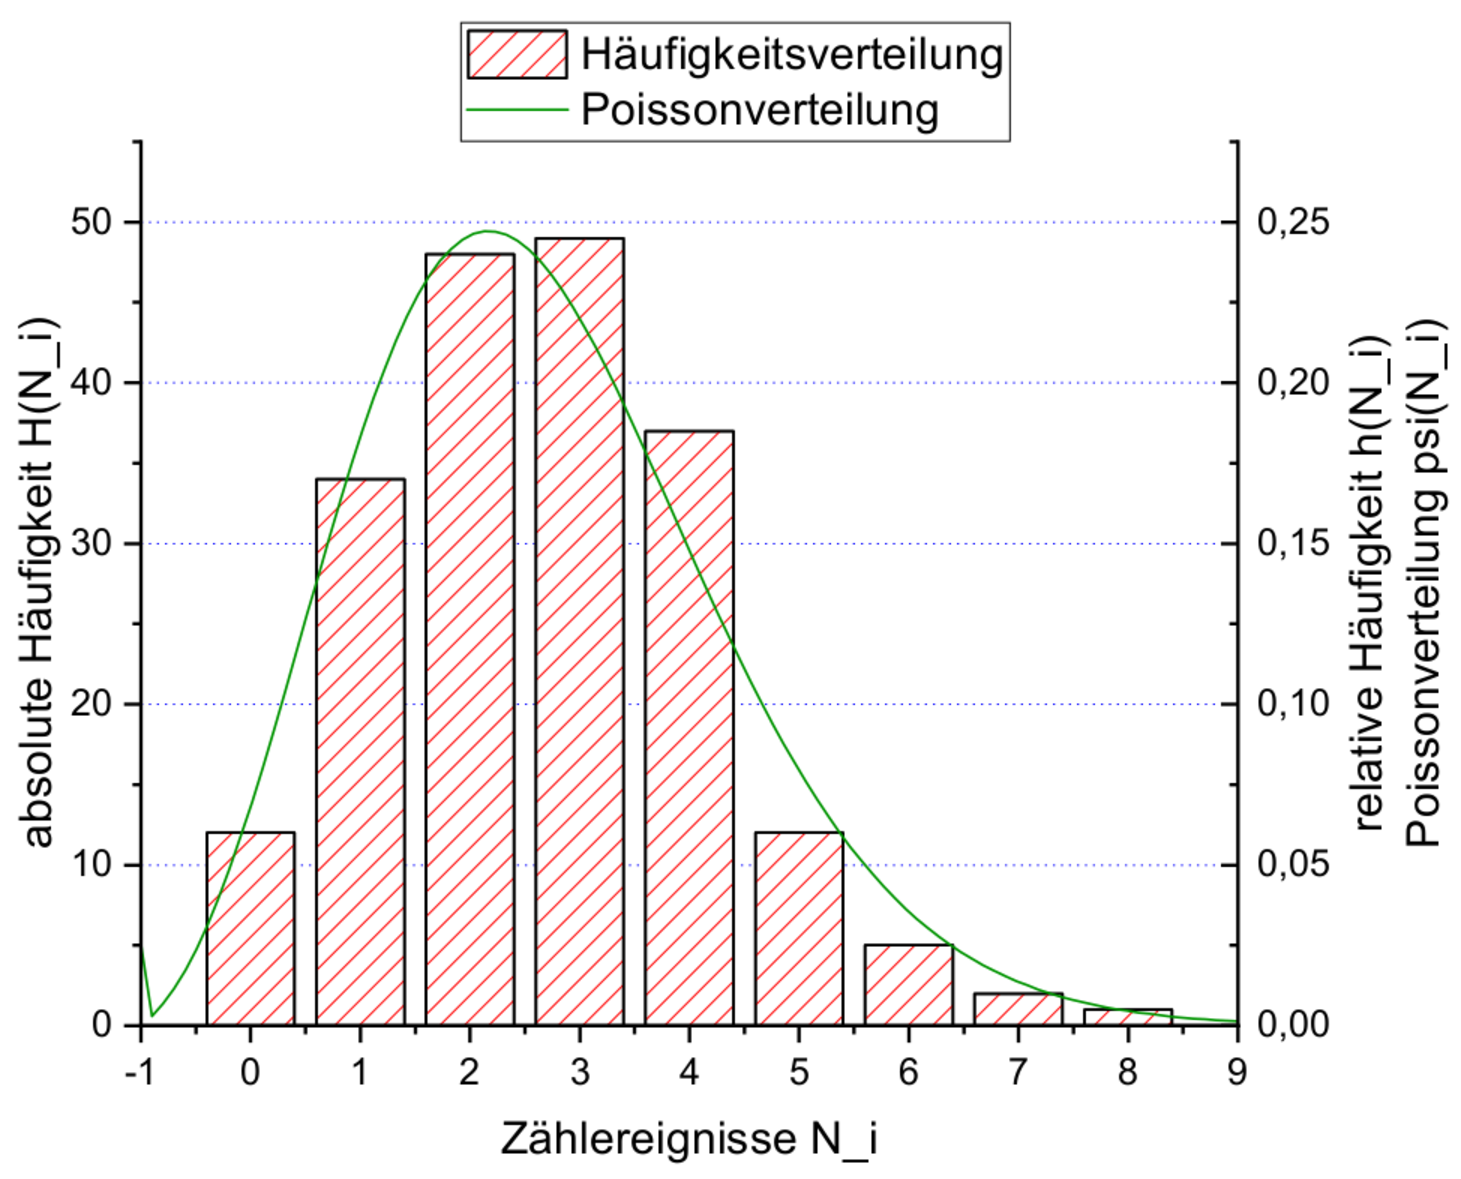
\includegraphics[width=0.7\textwidth]{Untergrund}
		\centering
		\caption{Aufgenommene absolute und relative Häufigkeitsverteilung der Untergrundpulse. Außerdem ist die durch deren Mittelwert festgelegte Poisson-Verteilung abgebildet.}%TODO Titel
		\label{Untergrund}
		\centering
	\end{figure}

	\subsubsection{Absorption von $\gamma$-Strahlung durch Blei} \label{blei}
	In \cref{GammaBlei} ist die Zählrate des $\gamma$-Präparats $ ^{137}$Cs logarithmisch gegen die Breite des Bleis aufgetragen. 
	Von der gemessenen Zählrate wurde die mittlere Untergrundaktivität \SI{0,2685}{Bq} abgezogen.
	Aus der Einführung ist bekannt, dass die Absorption von $\gamma$-Strahlung exponentiell zur Dicke ist.
	Mit:
	\begin{equation}
		a_{\gamma}(x) = a_{\gamma,0} \cdot exp(-\mu_\gamma x)= a_{\gamma,0} \cdot exp(-\mu_{\gamma,m} \rho x)
		\label{gamma}
	\end{equation}
	 Deshalb kann man bei einer logarithmischen Zählrate von einem linearen Zusammenhang zur Breite des Absorbers ausgehen. 
	 Entsprechend enthält \cref{GammaBlei} einen linearer Fit, aus dessen Steigung der Absorptionskoeffizient $\mu_\gamma$ bestimmt werden kann.
	 Aus $\mu_\gamma$ = $\SI{1,11 +- 0,04}{cm^{-1}}$ und der Dichte von Blei $\rho$ = $\SI{11,34}{g/cm^3}$ folgt ein Massenabsorptionskoeffizient $\mu_{\gamma,m}$ = $\SI{0,0978+-0,0035}{cm^2/g}$.\cite{dichten}
	 Die Absorptionskoeffizienten hängen von der Strahlungsenergie ab. 
	 Die hier bestimmten $\mu$ wurden bei einer $\gamma$-Strahlung mit einer Energie von ca. \SI{0,66}{MeV} gemessen.
	 
	\begin{figure}[H]
		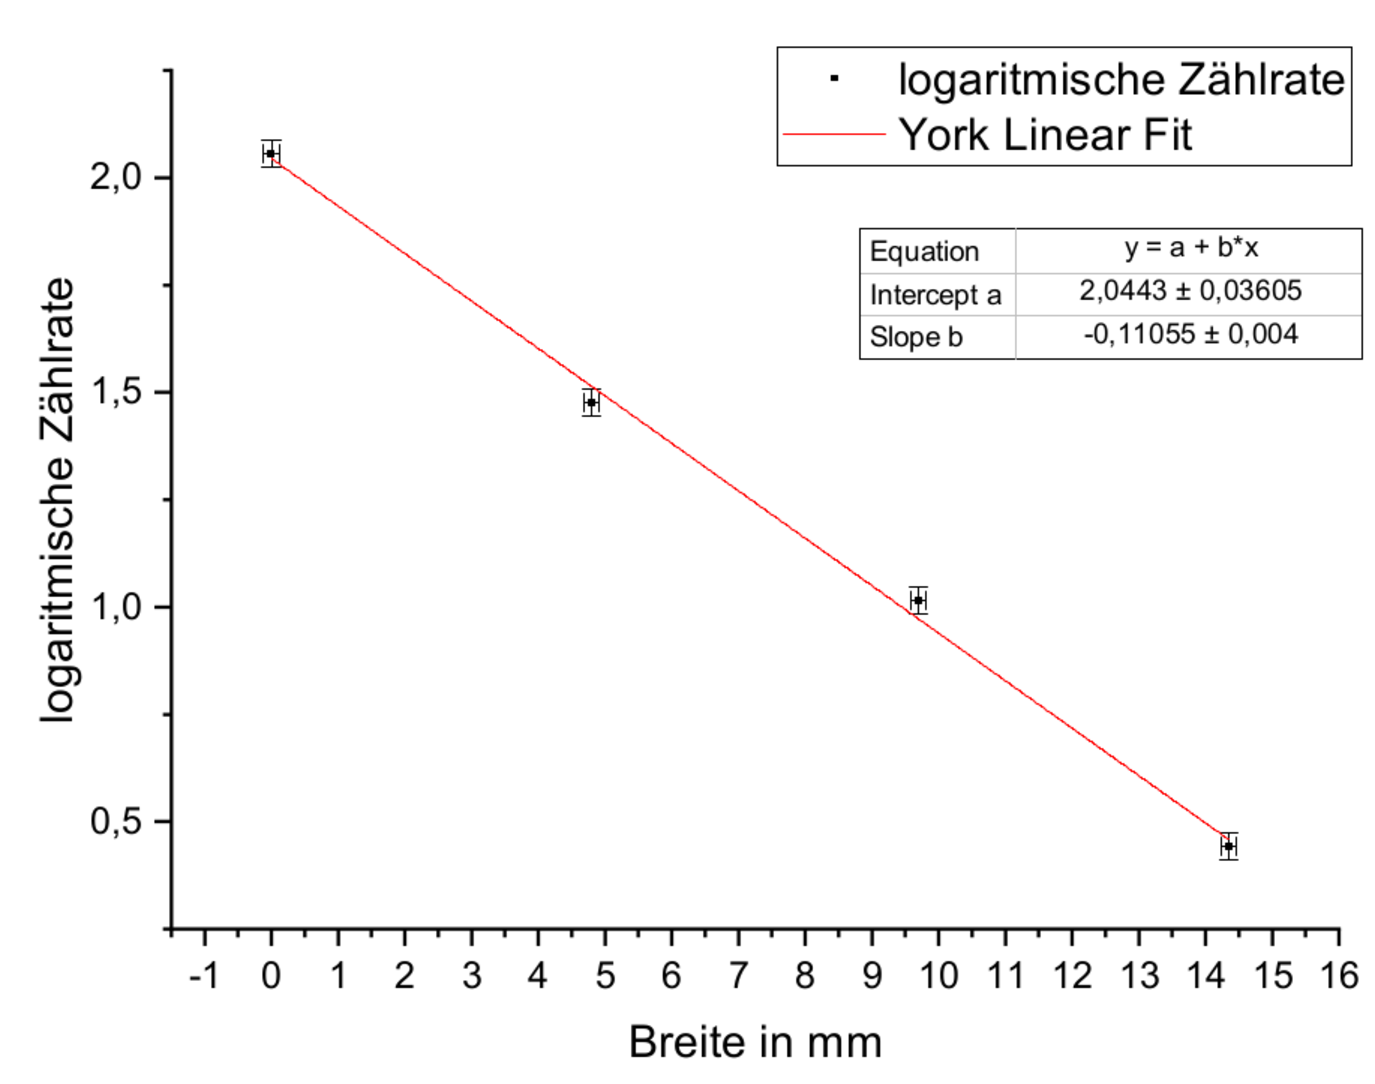
\includegraphics[width=0.7\textwidth]{GammaBlei}
		\centering
		\caption{Die Impulsrate ist logarithmisch gegen die Bleischichtdicke aufgetragen. Als $\gamma$-Präparat wurde $ ^{137}$Cs verwendet.}%TODO Titel
		\label{GammaBlei}
		\centering
	\end{figure}
	
	
	
	\subsubsection{Absorption von $\beta$-Strahlung} 
	Für die folgenden Rechnungen wurde wie in \cref{blei} beschrieben die Untergrundkorrektur durchgeführt.
	\subsubsection*{Aluminiumabsorber}
	
	Analog zu \cref{blei} lassen sich aus \cref{BetaAlu} Absorptions- und Massenabsorptionskoeffizient bestimmen. 
	Die exponentielle Näherung lässt sich auf den gesamten Bereich anwenden, da hier die logarithmische Zählrate linear zur Breite ist.
	Es ergeben sich $\mu_\beta$ = $\SI{19,5 +- 3,1}{cm^{-1}}$ und $\mu_{\beta,m}$ = $\SI{7,2+-1,1}{cm^2/g}$.\cite{dichten}
	\begin{figure}[H]
		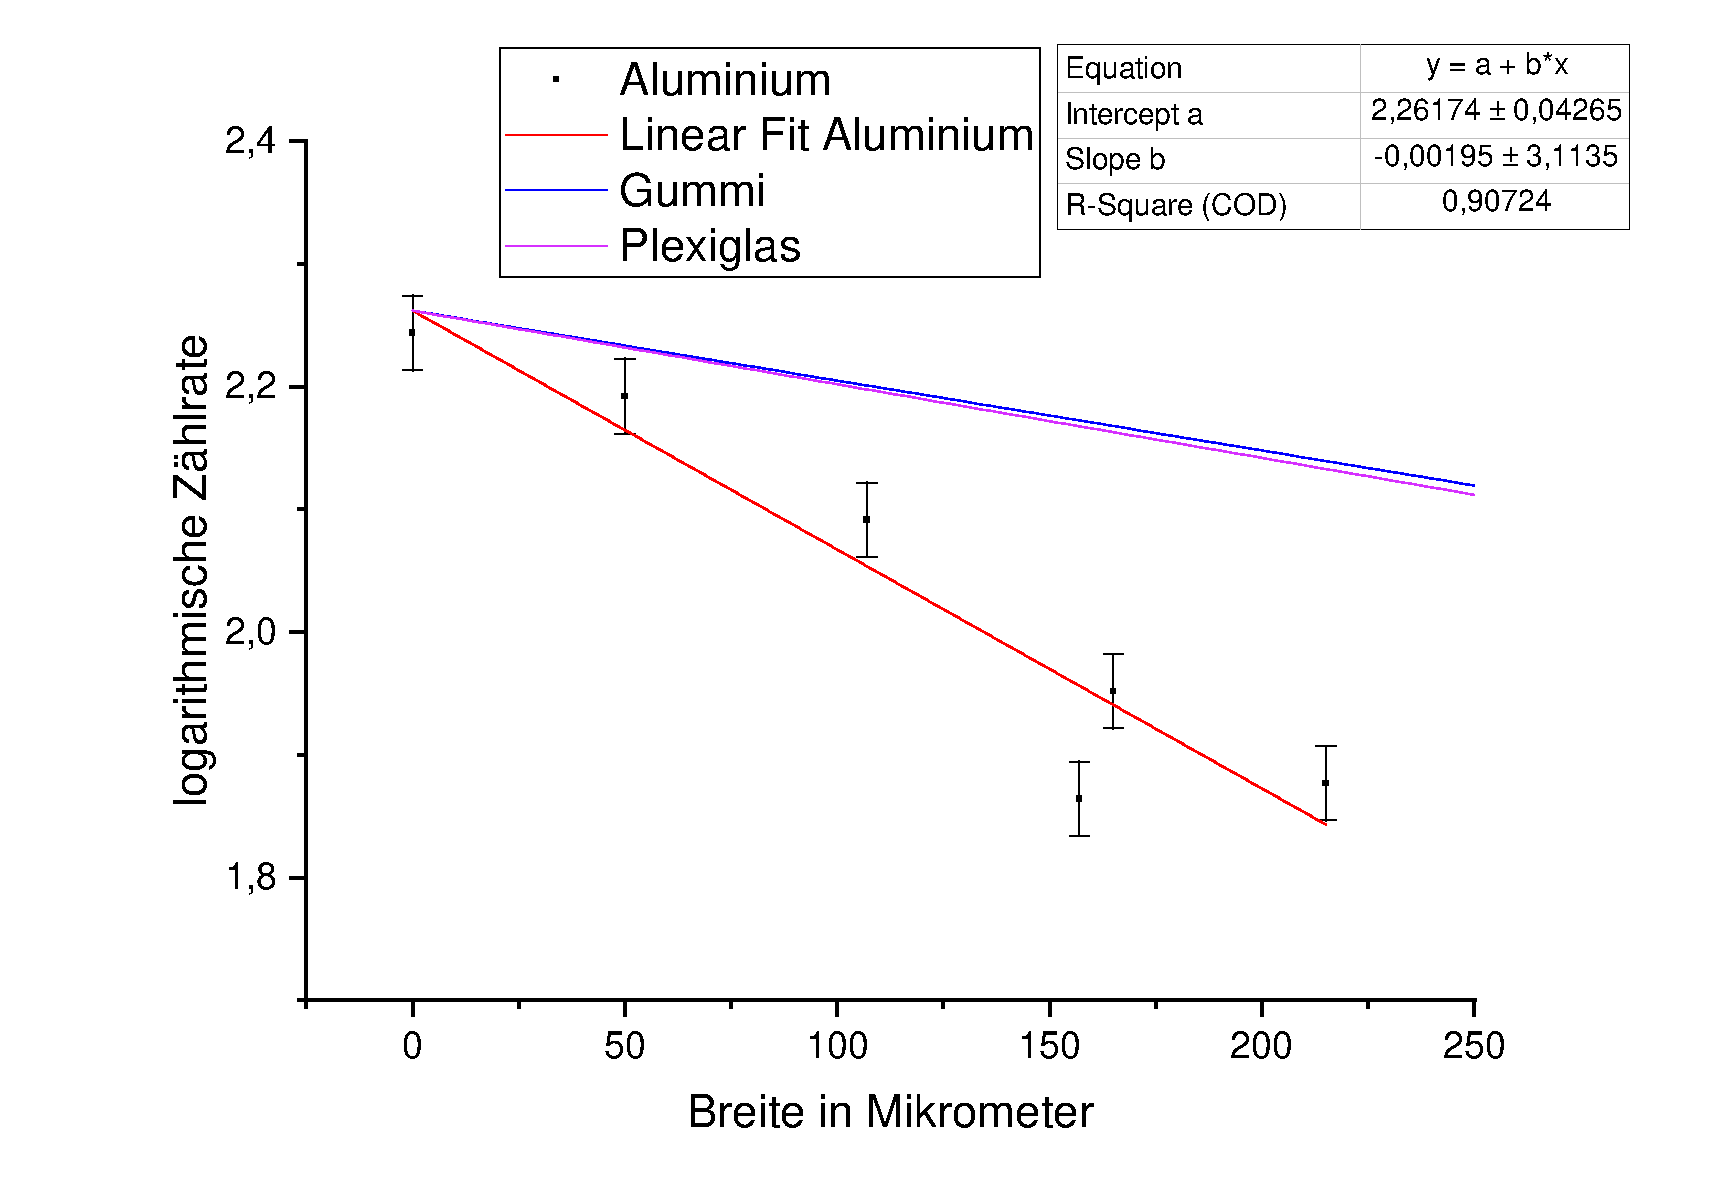
\includegraphics[width=0.7\textwidth]{BetaAlu}
		\centering
		\caption{Die Impulsrate ist logarithmisch gegen die Dicke des Absorbers aufgetragen. $ ^{90}$Sr diente als $\beta$-Präparat. Für das Aluminium wurden mehrere Messpunkte verwendet und ein linearer Fit ausgeführt. Für Gummi und Plexiglas wurde aus jeweils einem Messpunkt und der Zählrate ohne Absorber die Steigung der Geraden bestimmt.}
		\label{BetaAlu}
		\centering
	\end{figure}

	Einer der Messwerte befindet sich recht weit vom linearen Fit entfernt.
	
	\subsubsection*{Gummi- und Plexiglasabsorber} 
	Der Absorptionskoeffizient $\mu_\beta$ lässt sich analog zu $\mu_\gamma$ aus \cref{gamma} durch Umformen bestimmen.
	\begin{equation}
		\mu_\beta = \frac{\ln \left( \frac{a_{\beta,0}}{a_\beta(x)}\right)}{x}
	\end{equation}
	\begin{equation}
	u(\mu_\beta) = \sqrt{ \left(\frac{u(a_{\beta,0})}{a_{\beta,0}x}\right)^2 + \left(\frac{u(a_\beta(x))}{a_\beta(x)x}\right)^2 + \left(\frac{\mu_\beta u(x)}{x}\right)^2}
	\end{equation}
	In \cref{TabelleMu} sind die jeweiligen Parameter von Gummi und Plexiglas sowie das resultierende $\mu_\beta$ aufgeführt.
	Das $a_{\beta,0}$ beträgt \SI{9,43 +- 0,29}{Bq}.
	In \cref{BetaAlu} sind die Geraden für Gummi und Plexiglas mit dem jeweiligen $\mu_\beta$ dargestellt.
	\begin{table}[H]
		\centering
		\begin{tabular}{ c | c | c }
			&Gummi & Plexiglas \\ \hline
			$x$&\SI{2+-0,12}{mm}&\SI{4+-0,12}{mm}\\
			$a_\beta(x)$&\SI{3,02+-0,09}{Bq}&\SI{0,84+-0,03}{Bq}\\
			$\mu_\beta$&\SI{5,7+-0,4}{cm^{-1}}&\SI{6,0+-0,2}{cm^{-1}}\\
			
		\end{tabular}
		\caption{Aus Breite $x$ und Impulsrate $a_\beta(x)$ berechneter Absorptionskoeffizient von Gummi und Plexiglas.}
		\label{TabelleMu} 
	\end{table}
	
	\subsection{Diskussion}
	%TODO Bezug/Nutzten oder sonst was
	%TODO auch hier die Hypothese wiederholen
	%TODO keine Messwerte hier, nach manchen Menschen, zumindest "direkt" erstellte Diagramme net hier, auch wenn Lesbarkeit-bla
	Es ist ersichtlich, dass die Einsatzspannung des Zählrohrs zwischen 300 und \SI{325}{V} liegt. %lieber 2x SI?
	Auch das für Zählrohrkennlinien typische Plateau ist in \cref{Zaehlrohrcharakteristik} deutlich erkennbar.
	Der starke Anstieg vor dem Plateau konnte nicht aufgelöst werden und das Betriebsgerät verhinderte eine Erhöhung der Spannung auf Werte, die eine selbstständige Gasentladung zur Folge hätten.
	
	Die Annahme, dass das Auftragen der Häufigkeit gegen die Zählereignisse der Untergrundimpulse einer Poisson-Verteilung entspricht, ließ sich bestätigen, wie in \cref{Untergrund} deutlich zu erkennen ist.
	
	\subsubsection{Absorption von $\gamma$-Strahlung durch Blei}
	Literaturwerte geben für Strahlung mit $E=\SI{0,6}{MeV}$ ein $\mu_{\gamma,m}$ = $\SI{0,125}{cm^2/g}$ an (vgl.\cite{absorption_blei}).
	Dies deckt sich zwar nicht vollständig mit dem Messwert von \\
	$\mu_{\gamma,m} = $ \SI{0,0978 \pm 0,0035}{cm^2/g}, 
	aber dieser wurde auch nicht exakt bei $E$ = $\SI{0,6}{MeV}$ (sondern bei \SI{0,66}{MeV}) gemessen.
	Es lässt sich also zumindest die Größenordnung des Messwerts bestätigen.
	
	\subsubsection{Absorption von $\beta$-Strahlung}
	Das verwendete $\beta$-Präparat $^{90}$Sr zerfällt mit $E_{\beta,\text{max}}$= \SI{0,55}{MeV} in $^{90}$Y, welches mit $E_{\beta,\text{max}}$ = \SI{2,28}{MeV} in $^{90}$Zr übergeht (\cite{Einfuehrung}).
	Die Strahlung beider Zerfälle überlagert sich, jedoch überwiegt der Anteil des Tochternuklids $^{90}$Y. 
	Mithilfe der empirische Bleuler-Formel lässt sich die Reichweite der Elektronen abschätzen:
	\begin{equation}
	R_{\beta,\text{max}} \approx \frac{5,71 \cdot E_{\beta,\text{max}} - 1,61}{\rho}
	\label{Bleuler}
	\end{equation} %TODO cite http://www.chemie.de/lexikon/Blei.html
	Wobei $E_{\beta,\text{max}}$ in MeV und $\rho$ in $\text{kg/m}^3$ einzusetzen sind.
	Mit $E_{\beta,\text{max}}$= \SI{0,55}{MeV} und $\rho$= $\SI{2,7}{g/cm^3}$ folgt eine Maximale Reichweite von ca. \SI{550}{\micro\meter} für die Elektronen des Strontiumzerfalls durch Aluminium.
	
	\subsubsection*{Aluminiumabsorber}
	Aus dem linearen Zusammenhang in der logarithmischen Darstellung lässt sich erkennen, dass nur einer der Zerfälle einen messbaren Einfluss auf die Zerfallskurve hat, da sich ansonsten eine Überlagerung zweier Geraden unterschiedlicher Steigung in unterschiedlichen Bereichen der Schichtdicke ergeben hätte.
	Dies liegt vermutlich daran, dass sich das Präparat selbst nicht an der Oberfläche des Präparathalters, sondern hinter eine Abdeckung befand, die die niederenergetischen Elektronen des Strontiumzerfalls nicht durchdringen konnten.
	Insofern lässt sich erkennen, dass die Hypothese des näherungsweise exponentiellen Zusammenhangs im Messbereich von 0 bis \SI{215}{\micro \meter} bestätigt werden kann.
	
	Dass einer der Messwerte vom linearen Fit abweicht, lässt sich nur durch die stochastische Natur des Zerfallsprozesses und der Absorption erklären und der Fit liegt innerhalb der doppelten Unsicherheit des Messwerts.
	
	\subsubsection*{}
	Dass Gummi und Plexiglas einen geringeren Absorptionskoeffizienten als Aluminium haben, war aufgrund der geringeren Dichte zu erwarten.
	\par
	Würde man Blei als Absorber für die $\beta$-Strahlung wählen, wäre ein deutlich stärkerer Abfall der Impulsrate mit der Schichtdicke und eine geringere maximale Reichweite (\cref{Bleuler}) zu erwarten, da Blei eine höhere Dichte hat.
	Abhängig von der Schichtdicke wäre auch der exponentielle Abfall nicht mehr nachweisbar.
	%TODO Vergleich mu_beta einführungen mit unserem => Energieverteilung
	
	\section{Schlussfolgerung}
	%TODO Rückgriff auf Hypothese und drittes Nennen dieser
	Es ließen sich die Hypothesen im Wesentlichen bestätigen.
	Die Zählrohrcharakteristik zeigte den erwarteten Verlauf, nur der erneute Anstieg nach dem Plateau ließ sich nicht nachweisen, aber dies würde eine Zerstörung des Geiger-Müller-Zählrohrs nach sich ziehen, weshalb dieser Teil der Charakteristik schwer messbar ist.
	Die Untergrundstrahlung zeigte die erwartete Poisson-Verteilung bei der häufigen Messung kurzer Zeitintervalle.
	Auch die exponentielle Abnahme der Impulsrate von $\gamma$-Strahlung mit der Schichtdicke ließ sich zeigen und der daraus folgende Absorptionskoeffizient lag in der Größenordnung des Literaturwerts.
	
	Für die Untersuchung des $\beta$-Zerfalls wäre das Wissen, ob sich das Präparat auf der Oberfläche des Probenhalters oder hinter einer dünnen Abschirmung befindet, wichtig gewesen.
	Daraus, dass die Messergebnisse keine Überlagerung aus zwei Zerfällen unterschiedlicher Energien zeigten, lässt sich allerdings die begründete Vermutung ableiten, dass sich das Präparat in der Tat nicht direkt auf der Oberfläche befand.
	
	Hätte man beim $\beta$-Zerfall Schichtdicken, die größer als \SI{550}{\micro \meter} (nach \cref{Bleuler}) sind, gewählt, wären Elektronen aus dem energieärmeren Zerfall vollständig absorbiert worden, sodass man keine Überlagerung aus zwei Zerfällen in Betracht ziehen müsste.
	%TODO Quellen zitieren, Websiten mit Zugriffsdatum
	%TODO Verweise auf das Laborbuch (sind erlaubt)
	%TODO Tabelle + Bilder mit Beschriftung
	\printbibliography
\end{document}
